

\thispagestyle{empty}
\begin{tikzpicture}[remember picture, overlay]
\node[inner sep=0pt, xshift=.25\paperwidth, yshift=.25\paperheight] (vase) at (current page.south) {%
	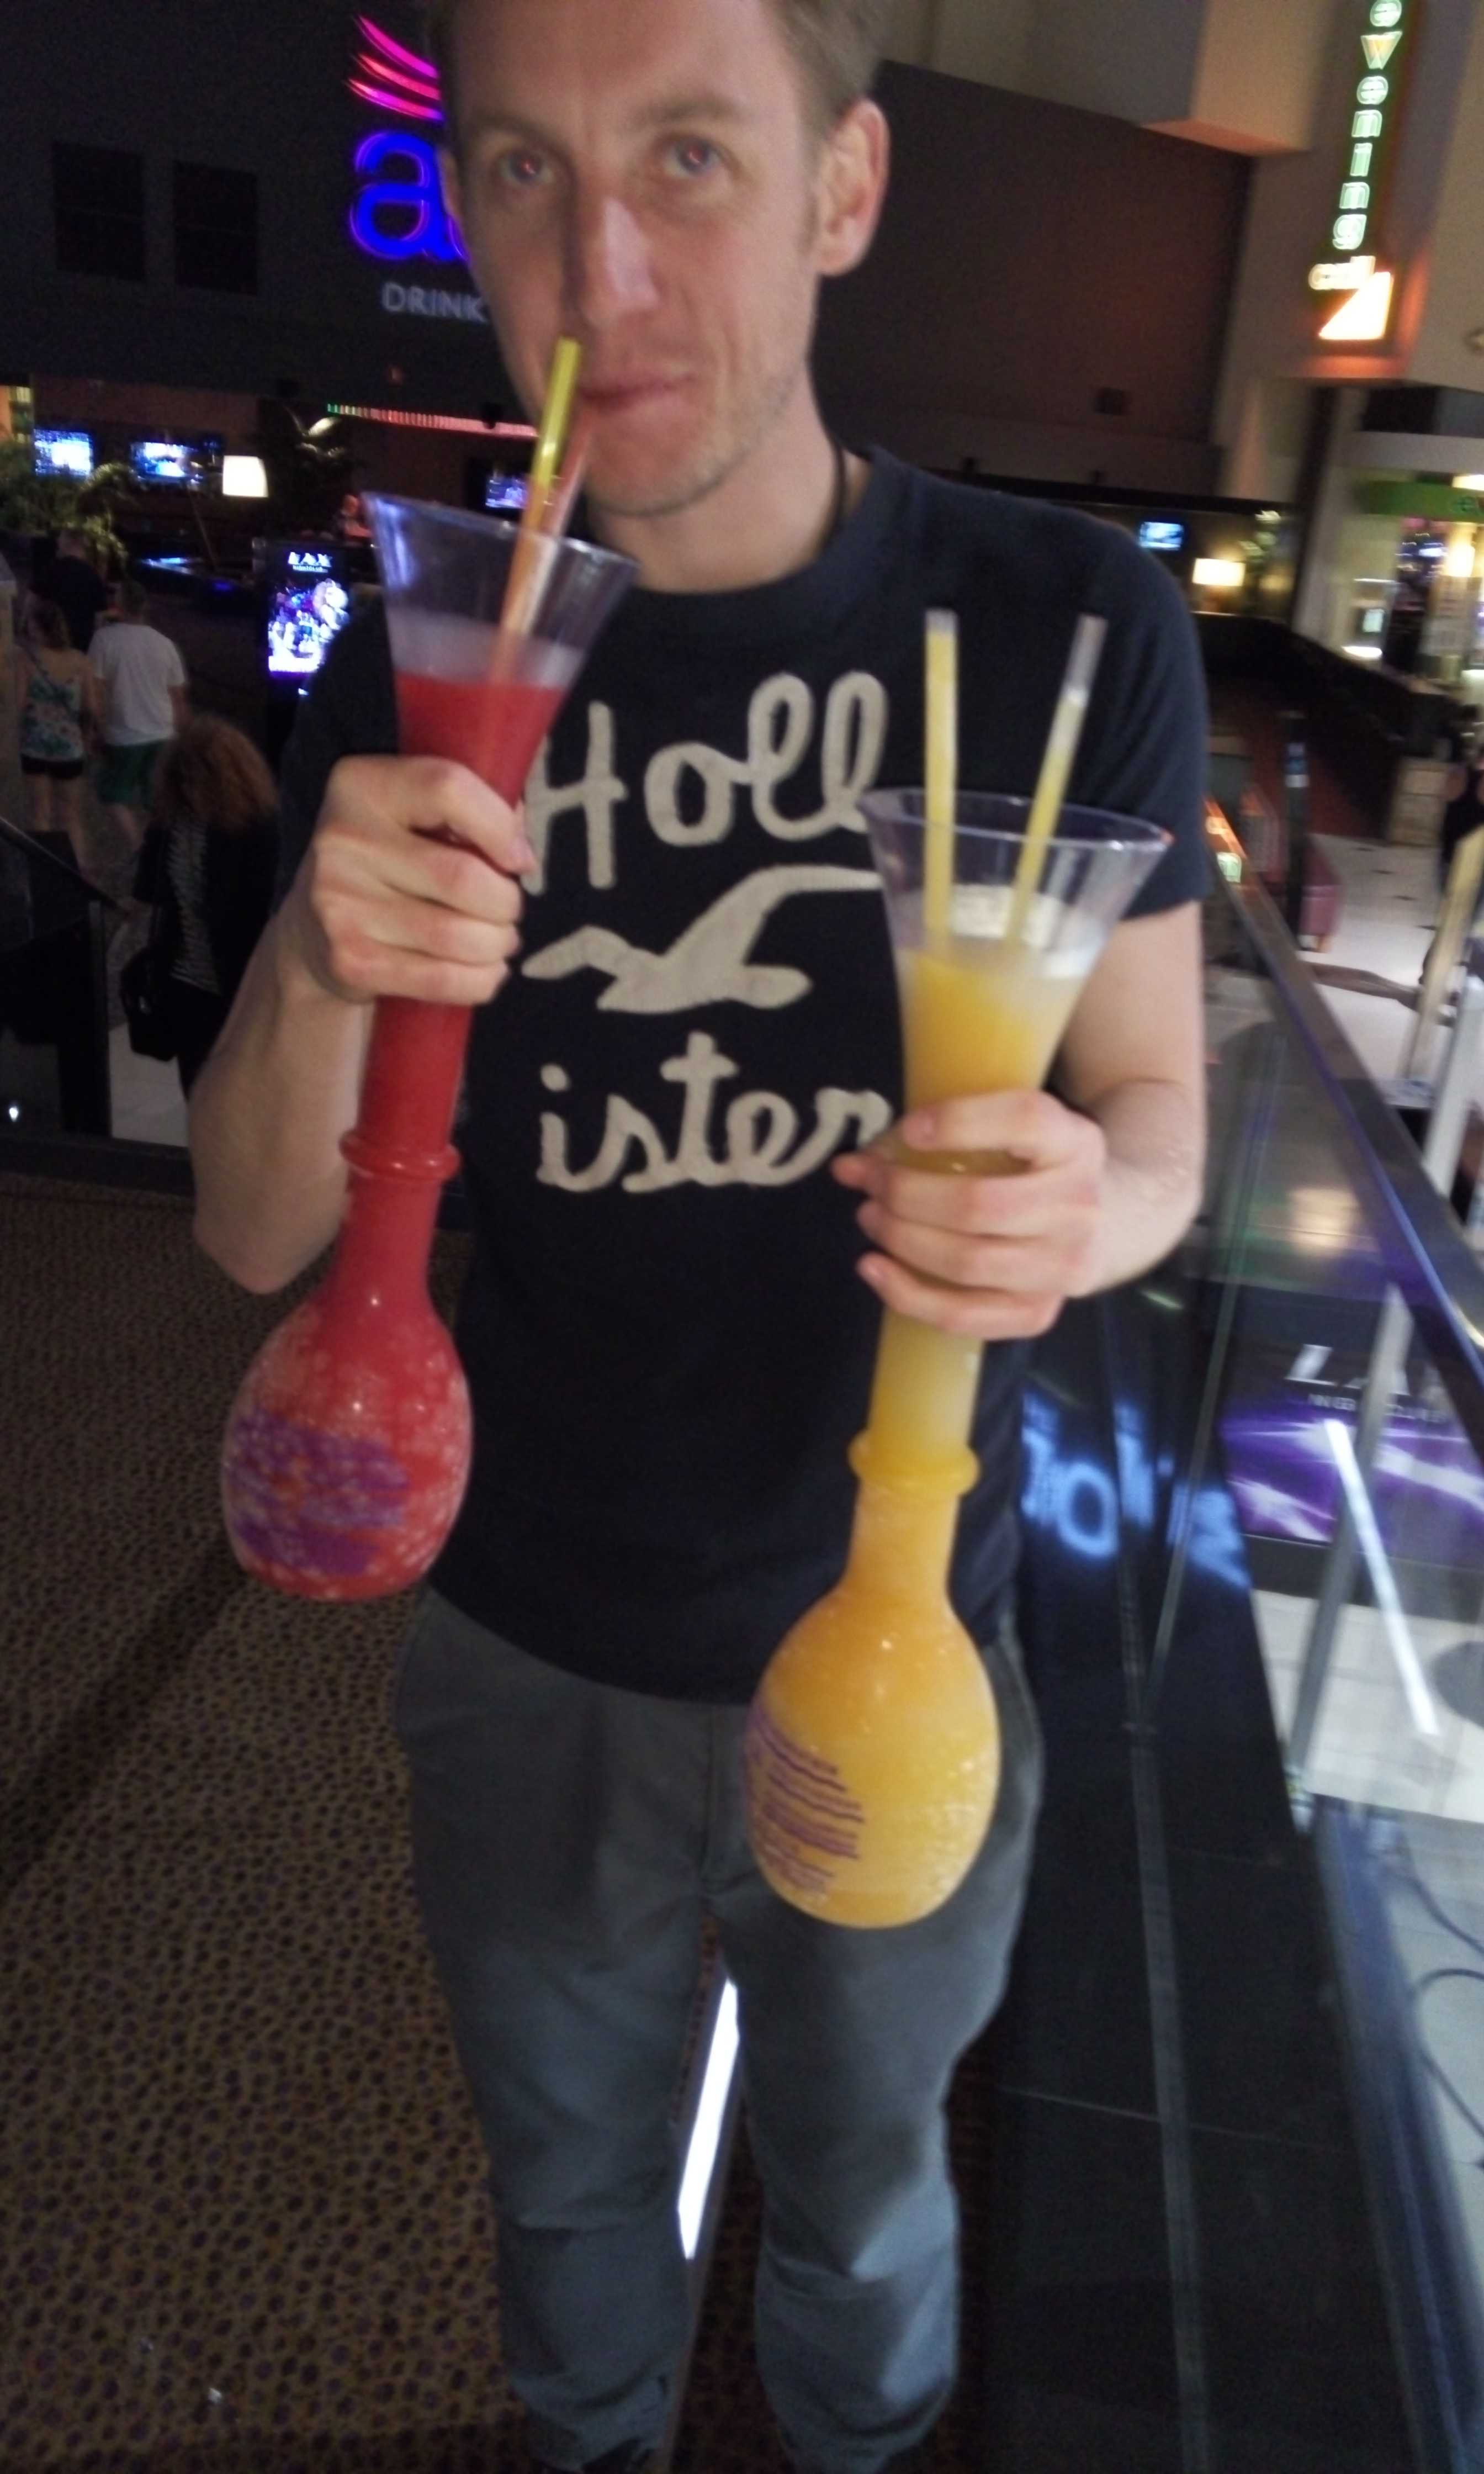
\includegraphics[width=.5\paperwidth,height=.5\paperheight]{11/image20160411_134402409.jpg};%
};
\node[inner sep=0pt, text width=.35\paperwidth, align=justify, xshift=-.2\paperwidth, yshift=1.2cm] at (vase.west) {%
	\FOREIGN{The Strip} war das Tagesprogramm.
	Den Boulevard sind wir auf der einen Seite hoch und auf der anderen Seite, mit ein bis zwei Vasen intus in leicht beeinflusster Gangart, wieder herunter gelaufen.
	Die einzelnen Hotels haben verschiedene Mottos und jedes ist dann doch irgendwie beeindruckend!
	
	Wenn man dann weiß, dass der Großteil der Hotels dem Hollywood Filmstudio MGM gehört, erscheinen die hier spielenden Filme (Ocean 11\dots 13, Hangover 1\dots 3, \dots) in einem anderen Licht.
};
%  \node[black,fill=white,text width=10em] (blub) at (0.5,0) {Distanz etwa 3.600~km}; %
\end{tikzpicture}

\newpage

%\vspace*{1cm}

Der Vaseninhalt ist alkoholhaltiges Squash-/Wassereis und besteht in erster Linie aus billigstem Fusel.
Vom vielen Laufen und anderem sind wir gegen Abend angeknockt mal kurz ins Bett gefallen und nach zwei statt der vorgenommenen einen Stunde unter größter Überwindung wieder aufgerumpelt.
Wir wollten noch etwas Essen und das beim Herumlaufen gefundene \FOREIGN{BeerHaus} klang vielversprechend.
Das Essen war weder berauschend noch gut, es füllte nur den Magen.
Die Wirkung der Vasen setzte uns weiterhin kräftig zu und wir liefen zurück ins Hotel.

Auf dem Heimweg wurde uns noch Coke angeboten, aber zu dem Zeitpunkt hatten wir beide schon die Schnauze voll von Gesellschaftsdrogen.
Ein anderer Geschäftsmann sprach uns noch wie folgt an.
\begin{quote}
	\FOREIGN{Want some titties tonight?}
\end{quote}
Was ich verneinte und er daraufhin sein Angebot erhöhte.
\begin{quote}
	\FOREIGN{They are wrapped in bacon!}
\end{quote}
Zu seinem Pech kamen wir gerade vom Essen und wollten nur noch irgendwie durch den aus Spielautomaten und -tischen bestehenden Irrgarten im Erdgeschoss unseres Hotels.
